\documentclass[10pt]{article}
\usepackage{icmlko}

\icmlmeta{IP 파운데이션 월드모델}{168}{아홉 중 여덟이 차트에서 나왔다}{표본을 어떻게 뽑았는지가 백예순여덟 노트 동안 어디에도 안 적혀 있었다. 코드에서 읽어 적었더니 노트 167의 점프가 설명된다}

\begin{document}

\twocolumn[
\icmlheader

\begin{abstract}
노트 167이 제작 주체 이력 축의 효과가 통째로 ``0건 대 1건 이상''의 점프임을
보이고(6/6 양수, 평균 $+$0.132, 1건 이상 안에서는 $-$0.015) 그 원인으로
표본 선택을 지목했다. 그런데 \textbf{도메인마다 표본을 어떻게 뽑았는지가
어디에도 안 적혀 있었다} --- 모듈 머리말은 왜 그 도메인을 골랐는지만 적고
어떻게 골랐는지는 수집 코드 안에 있었다. 읽어서 적었다.
\textbf{아홉 중 여덟이 인기 정렬 표본이다.} 게임은 Steam
\texttt{filter=topsellers}, 모바일은 App Store
\texttt{top\{free,paid,grossing\}} 차트, 도서는 알라딘 베스트셀러 페이지,
만화 · 세계애니는 AniList \texttt{sort: POPULARITY\_DESC}, 웹툰은 네이버
\texttt{order=user}, 애니 · 아이돌은 부분적으로 순위 지표를 섞는다.
\textbf{펀딩만 아니다} --- 텀블벅 목록을 페이지 순서대로 훑어 종료된
프로젝트를 담는다. 그리고 그 하나가 \textbf{노트 167에서 점프가 없던 유일한
도메인}이다. 펀딩을 다른 일곱과 같은 방식(표본 안 계수)으로 다시 세면
$-$0.005이고 0건 대 1건 이상의 라벨 중앙값이 1.959 대 1.924로 차이가 없다.
반면 차트 표본 여섯은 $+$0.058$\sim$$+$0.312로 전부 점프가 있다.
\textbf{인기 정렬 표본에서 ``표본 안에 앞선 작품이 있다''는 ``앞서 히트를
냈다''는 뜻이고, 그래서 점프가 생긴다.} 어느 축이 걸리는지도 적었다 ---
표본 안 계수를 쓰는 것은 \texttt{venue\_prominence}(일곱 도메인)와
\texttt{media\_push}(아이돌 · 게임)이고, 나머지 셋은 레코드 자체의
속성이라 안 걸린다. \textbf{노트 163에서 손잡이 정확도 100\% · 98\%로
제일 높았던 타깃 폭과 굿즈 규모가 정확히 그 안 걸리는 셋에 있다.}
\end{abstract}
]

\begin{figure*}[t]
\centering
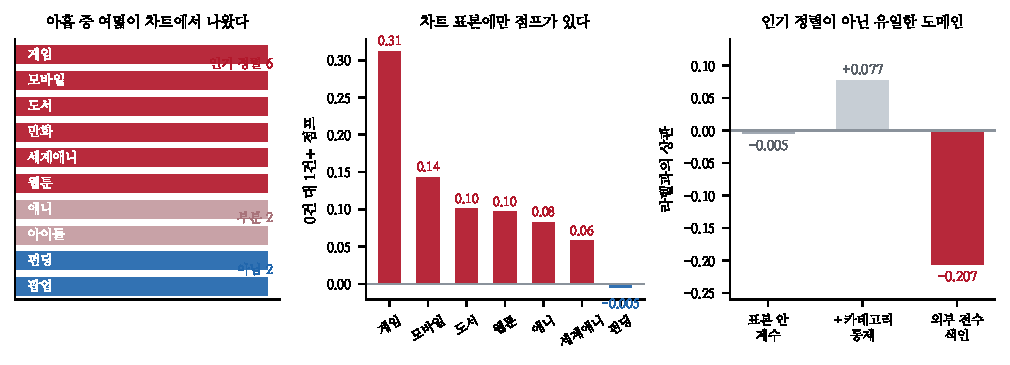
\includegraphics[width=\textwidth]{figs/sample.pdf}
\caption{왼쪽 --- 아홉 중 여덟이 차트에서 나왔다. 가운데 --- 차트 표본에만
점프가 있다. 오른쪽 --- 인기 정렬이 아닌 유일한 도메인.}
\end{figure*}

\section{어디에도 안 적혀 있었다}

\begin{table}[t]
\centering\tsize
\caption{수집 코드에서 읽은 표본 뽑기.}
\begin{tabular}{lll}
\toprule
& 뽑는 법 & 인기? \\
\midrule
게임 & Steam \texttt{topsellers} & ○ \\
모바일 & App Store 차트 & ○ \\
도서 & 알라딘 베스트셀러 & ○ \\
만화 & AniList \texttt{POPULARITY\_DESC} & ○ \\
세계애니 & AniList 같은 방식 & ○ \\
웹툰 & 네이버 \texttt{order=user} & ○ \\
애니 & 라프텔 \texttt{recent}$+$\texttt{rank} & 부분 \\
아이돌 & 차트 지표 포함 & 부분 \\
\textbf{펀딩} & \textbf{텀블벅 목록 순차} & \textbf{×} \\
팝업 & 계약 기록 $+$ 시장 레코드 & × \\
\bottomrule
\end{tabular}
\end{table}

\claimx{\textbf{아홉 중 여덟이 인기 정렬이다.} 도메인을 늘릴 때마다 ``라벨이
같은 물리량인가''는 매번 따졌는데(모듈 머리말이 전부 그 얘기다) ``어떻게
뽑았나''는 한 번도 안 적었다.}{나쁜 선택이었다는 뜻은 아니다 --- 차트는
API 가 그대로 주는 것이고 표본을 만드는 제일 싼 길이다. \textbf{안 적은
것이 문제다.}}

\section{그 하나가 점프가 없다}

\begin{table}[t]
\centering\tsize
\caption{0건 대 1건 이상의 점프(노트 167).}
\begin{tabular}{lrl}
\toprule
게임 & $+$.312 & 차트 \\
모바일 & $+$.143 & 차트 \\
도서 & $+$.101 & 차트 \\
웹툰 & $+$.097 & 차트 \\
애니 & $+$.083 & 부분 \\
세계애니 & $+$.058 & 차트 \\
\midrule
\textbf{펀딩} & \textbf{$-$.005} & \textbf{차트 아님} \\
\bottomrule
\end{tabular}
\end{table}

\claimx{\textbf{차트 표본 여섯은 전부 점프가 있고 차트가 아닌 하나는
없다.} 펀딩의 0건 대 1건 이상 라벨 중앙값이 1.959 대 1.924로 차이가
없다.}{도메인 일곱의 관측이고 ``차트 아님''이 하나뿐이다. 인과 주장에는
약하지만 \textbf{예측이 맞은 것}이다 --- 노트 167에서 표본 선택을 지목하고
이 노트에서 확인했다.}

\claimx{\textbf{읽는 법.} 인기 정렬 표본에서 ``표본 안에 앞선 작품이
있다''는 곧 ``앞서 히트를 냈다''는 뜻이다. 그러니 점프는 창작자가 부지런한
정도가 아니라 \emph{앞선 성공}을 잰다.}{그 정보 자체는 오픈 전에 알 수
있고 라벨 누수도 아니다(이 작품이 아니라 이전 작품들의 결과다). 다만
축 이름과 손잡이 해석이 달라진다 --- 노트 167의 결론 그대로다.}

\section{어느 축이 걸리나}

\begin{table}[t]
\centering\tsize
\caption{표본 안 계수를 쓰는 축.}
\begin{tabular}{lll}
\toprule
축 & 도메인 & 노트 163 정확도 \\
\midrule
\texttt{venue\_prominence} & 일곱 & 74\% \\
\texttt{media\_push} & 아이돌 · 게임 & 75\% \\
\midrule
\texttt{target\_breadth} & --- & \textbf{100\%} \\
\texttt{goods\_scale} & --- & \textbf{98\%} \\
\texttt{entry\_friction} & --- & 68\% \\
\bottomrule
\end{tabular}
\end{table}

\claimx{\textbf{손잡이 정확도가 제일 높았던 둘이 정확히 안 걸리는 축이다.}
타깃 폭(100\%)과 굿즈 규모(98\%)는 레코드 자체의 속성이라 표본 뽑기와
무관하다. 걸리는 둘은 74\% · 75\%다.}{입장 마찰(68\%)도 안 걸리는데
제일 낮다 --- 그러니 ``표본 안 계수''가 낮은 정확도의 유일한 원인은
아니다. 노트 164가 잰 구성물 수(입장 마찰 넷)가 그쪽 설명이다.}

\section{남기는 것}

\texttt{docs/SAMPLING.md} 에 표본 뽑기를 도메인마다 적었고
\texttt{docs/AXIS\_MEANING.md} 와 나란히 둔다. 노트 164가 ``슬롯에 무엇이
들었나''를 적었고 이 노트가 ``그 값이 어디서 왔나''를 적는다.

\claimx{\textbf{규약: 표본 안 계수를 축으로 쓸 때는 그 도메인의 표본
뽑기를 같이 적는다.}}{되돌리자는 것이 아니다. 노트 166이 잰 대로 이 축을
슬롯에서 꺼내는 것만으로 판이 $-$0.0104 내려간다 --- \textbf{쓰되 무엇인지
알고 쓰자}는 것이다.}

\begin{table}[t]
\centering\tsize
\caption{남은 것.}
\begin{tabular}{ll}
\toprule
\textbf{이진화} & 점프뿐이라면 이진 표지로 바꾸면 어떻게 되나 \\
전수 색인 & 게임 · 모바일은 API 로 전수를 셀 수 있다 \\
표본 확장 & 차트 밖을 섞으면 점프가 줄어드나 \\
\bottomrule
\end{tabular}
\end{table}

첫 줄이 곧바로 잴 수 있다. 효과가 0 대 1$+$ 점프뿐이라면 $\log_2(n{+}1)$
눈금을 쓸 이유가 없다. \textbf{이진으로 바꾸면 판이 어떻게 되는지}가
다음이고, 안 내려가면 축의 뜻이 코드에서도 정직해진다.

\end{document}
